\PassOptionsToPackage{unicode=true}{hyperref} % options for packages loaded elsewhere
\PassOptionsToPackage{hyphens}{url}
%
\documentclass[ignorenonframetext,]{beamer}
\usepackage{pgfpages}
\setbeamertemplate{caption}[numbered]
\setbeamertemplate{caption label separator}{: }
\setbeamercolor{caption name}{fg=normal text.fg}
\beamertemplatenavigationsymbolsempty
% Prevent slide breaks in the middle of a paragraph:
\widowpenalties 1 10000
\raggedbottom
\setbeamertemplate{part page}{
\centering
\begin{beamercolorbox}[sep=16pt,center]{part title}
  \usebeamerfont{part title}\insertpart\par
\end{beamercolorbox}
}
\setbeamertemplate{section page}{
\centering
\begin{beamercolorbox}[sep=12pt,center]{part title}
  \usebeamerfont{section title}\insertsection\par
\end{beamercolorbox}
}
\setbeamertemplate{subsection page}{
\centering
\begin{beamercolorbox}[sep=8pt,center]{part title}
  \usebeamerfont{subsection title}\insertsubsection\par
\end{beamercolorbox}
}
\AtBeginPart{
  \frame{\partpage}
}
\AtBeginSection{
  \ifbibliography
  \else
    \frame{\sectionpage}
  \fi
}
\AtBeginSubsection{
  \frame{\subsectionpage}
}
\usepackage{lmodern}
\usepackage{amssymb,amsmath}
\usepackage{ifxetex,ifluatex}
\usepackage{fixltx2e} % provides \textsubscript
\ifnum 0\ifxetex 1\fi\ifluatex 1\fi=0 % if pdftex
  \usepackage[T1]{fontenc}
  \usepackage[utf8]{inputenc}
  \usepackage{textcomp} % provides euro and other symbols
\else % if luatex or xelatex
  \usepackage{unicode-math}
  \defaultfontfeatures{Ligatures=TeX,Scale=MatchLowercase}
\fi
\usetheme[]{metropolis}
% use upquote if available, for straight quotes in verbatim environments
\IfFileExists{upquote.sty}{\usepackage{upquote}}{}
% use microtype if available
\IfFileExists{microtype.sty}{%
\usepackage[]{microtype}
\UseMicrotypeSet[protrusion]{basicmath} % disable protrusion for tt fonts
}{}
\IfFileExists{parskip.sty}{%
\usepackage{parskip}
}{% else
\setlength{\parindent}{0pt}
\setlength{\parskip}{6pt plus 2pt minus 1pt}
}
\usepackage{hyperref}
\hypersetup{
            pdfborder={0 0 0},
            breaklinks=true}
\urlstyle{same}  % don't use monospace font for urls
\newif\ifbibliography
\setlength{\emergencystretch}{3em}  % prevent overfull lines
\providecommand{\tightlist}{%
  \setlength{\itemsep}{0pt}\setlength{\parskip}{0pt}}
\setcounter{secnumdepth}{0}

% set default figure placement to htbp
\makeatletter
\def\fps@figure{htbp}
\makeatother


\title{Small area estimation of district-level fertility in sub-Saharan Africa}
\author{Oli Stevens\\
Imperial College London}
\date{6th April 2020}

\begin{document}
\frame{\titlepage}

\begin{frame}[t]{Introduction \textbar{} Background}
\protect\hypertarget{introduction-background}{}

\begin{itemize}
\tightlist
\item
  UNAIDS Reference Group for Estimates, Modelling and Projections
  provides technical recommendations to UNAIDS for the creation of
  annual HIV estimates
\item
  Newly created subnational estimation model - Naomi

  \begin{itemize}
  \tightlist
  \item
    District-level estimates of prevalence, incidence, ART coverage by
    sex and 5 year age groups
  \end{itemize}
\end{itemize}

\end{frame}

\begin{frame}[t]{Introduction \textbar{} Background}
\protect\hypertarget{introduction-background-1}{}

\begin{itemize}
\tightlist
\item
  UNAIDS Reference Group for Estimates, Modelling and Projections
  provides technical recommendations to UNAIDS for the creation of
  annual HIV estimates
\item
  Newly created subnational estimation model - Naomi

  \begin{itemize}
  \tightlist
  \item
    District-level estimates of prevalence, incidence, ART coverage by
    sex and 5 year age groups
  \end{itemize}
\end{itemize}

\begin{center}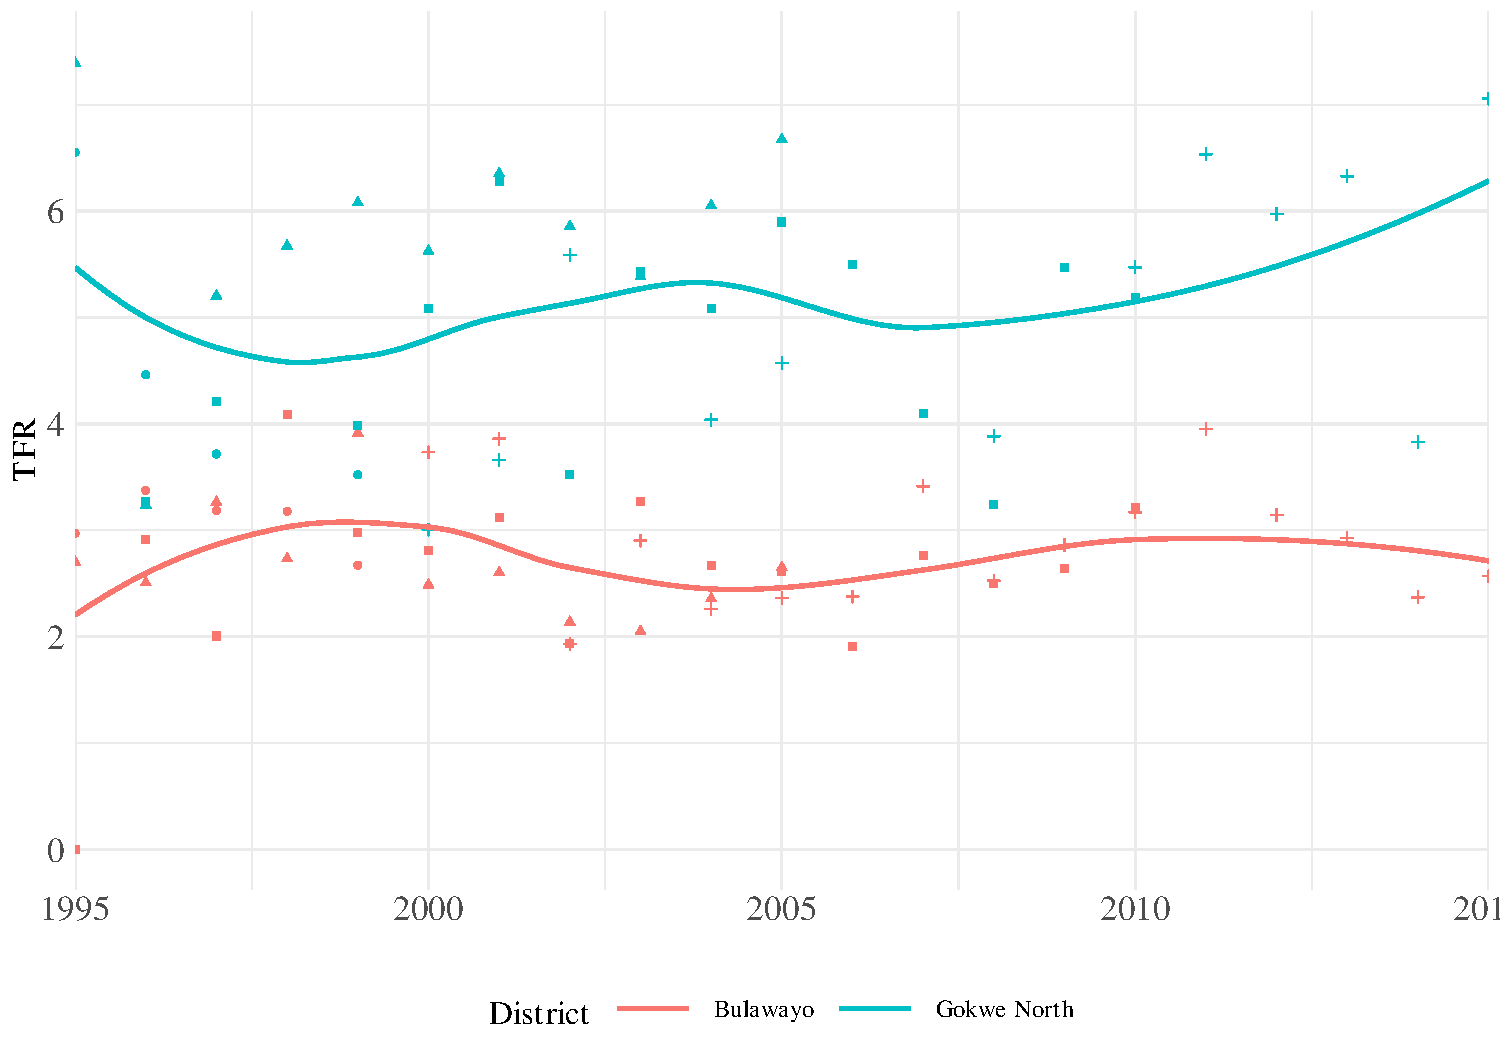
\includegraphics[height=0.5\textheight]{2020_04_UNPD_files/figure-beamer/unnamed-chunk-1-1} \end{center}

\end{frame}

\begin{frame}[t]{Introduction \textbar{} Background}
\protect\hypertarget{introduction-background-2}{}

\begin{itemize}
\tightlist
\item
  UNAIDS Reference Group for Estimates, Modelling and Projections
  provides technical recommendations to UNAIDS for the creation of
  annual HIV estimates
\item
  Newly created subnational estimation model - Naomi

  \begin{itemize}
  \tightlist
  \item
    District-level estimates of prevalence, incidence, treatment
    coverage by sex and 5 year age groups
  \end{itemize}
\item
  District level estimates of fertility desired for:

  \begin{itemize}
  \tightlist
  \item
    Estimation of children living with HIV

    \begin{itemize}
    \tightlist
    \item
      Key epidemic indicator
    \item
      Resource allocation for prevention of mother-to-child transmission
    \end{itemize}
  \item
    Improved projections at district level
  \end{itemize}
\end{itemize}

\end{frame}

\begin{frame}[t]{Data and workflow \textbar{} Zimbabwe}
\protect\hypertarget{data-and-workflow-zimbabwe}{}

\begin{itemize}
\tightlist
\item
  Demographic Health Surveys

  \begin{itemize}
  \tightlist
  \item
    Geomasked coordinates assigned to district
  \item
    1999, 2005, 2010, 2015
  \end{itemize}
\item
  Multiple Indicator Cluster Survey

  \begin{itemize}
  \tightlist
  \item
    Survey region indicator
  \item
    2009, 2014, 2019
  \end{itemize}
\item
  Birth history data:

  \begin{itemize}
  \tightlist
  \item
    DHS, MICS: 15 years
  \item
    (Malaria Indicator Survey/AIDS Indicator Surveys): 5 years
  \end{itemize}
\end{itemize}

\end{frame}

\begin{frame}[t]{Data and workflow \textbar{} Zimbabwe}
\protect\hypertarget{data-and-workflow-zimbabwe-1}{}

\begin{itemize}
\tightlist
\item
  R packages \emph{rdhs} and \emph{demogsurv}
\item
  Reconstruct survey-weighted births and observed person years, by
  single year, 5 year age groups, and district

  \begin{itemize}
  \tightlist
  \item
    CMC respondent's birth
  \item
    CMC respondent's births
  \item
    CMC interview
  \end{itemize}
\end{itemize}

\end{frame}

\begin{frame}[t]{Data and workflow \textbar{} Non-sampling bias in
household surveys}
\protect\hypertarget{data-and-workflow-non-sampling-bias-in-household-surveys}{}

\begin{itemize}
\tightlist
\item
  DHS collects full birth histories for children in the previous 5
  years, and an abbreviated question set thereafter
\item
  Interviewers can reduce workload by:

  \begin{itemize}
  \tightlist
  \item
    Displacing
  \item
    Omitting
  \end{itemize}
\end{itemize}

\end{frame}

\begin{frame}[t]{Data and workflow \textbar{} Non-sampling bias in
household surveys}
\protect\hypertarget{data-and-workflow-non-sampling-bias-in-household-surveys-1}{}

\begin{itemize}
\tightlist
\item
  DHS collects full birth histories for children in the previous 5
  years, and an abbreviated question set thereafter
\item
  Interviewers can reduce workload by:

  \begin{itemize}
  \tightlist
  \item
    Displacing
  \item
    Omitting
  \end{itemize}
\end{itemize}

\begin{center}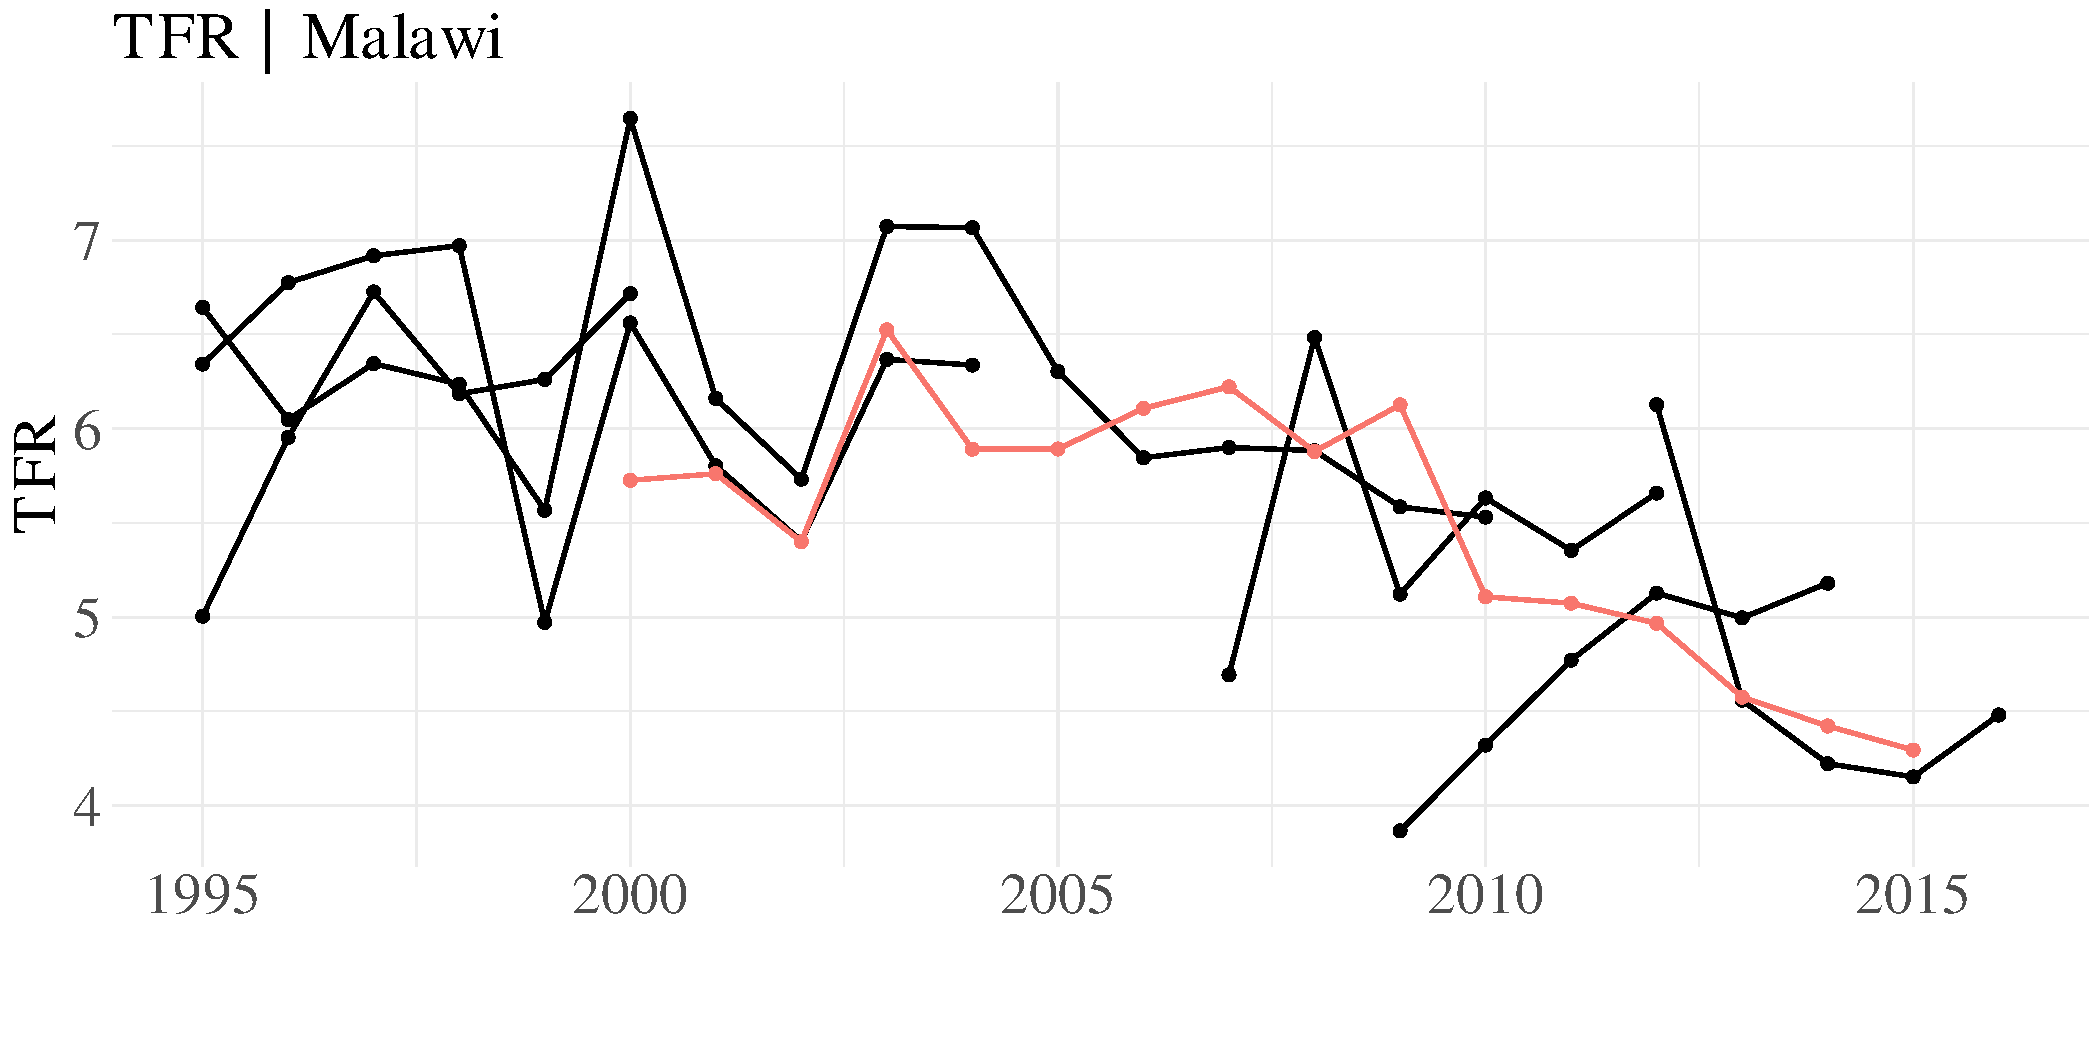
\includegraphics[height=0.5\textheight]{2020_04_UNPD_files/figure-beamer/unnamed-chunk-3-1} \end{center}

\end{frame}

\begin{frame}[t]{Data and workflow \textbar{} Non-sampling bias in
household surveys}
\protect\hypertarget{data-and-workflow-non-sampling-bias-in-household-surveys-2}{}

\begin{itemize}
\tightlist
\item
  Intersurvey analysis can estimate magnitude of bias due to overlap in
  recall periods

  \begin{itemize}
  \tightlist
  \item
    Many countries within SSA have surveys of moderate or poor quality
  \end{itemize}
\end{itemize}

\end{frame}

\begin{frame}[t]{Data and workflow \textbar{} Non-sampling bias in
household surveys}
\protect\hypertarget{data-and-workflow-non-sampling-bias-in-household-surveys-3}{}

\begin{itemize}
\tightlist
\item
  Intersurvey analysis can estimate magnitude of bias due to overlap in
  recall periods

  \begin{itemize}
  \tightlist
  \item
    Many countries within SSA have surveys of moderate or poor quality
  \end{itemize}
\end{itemize}

\begin{center}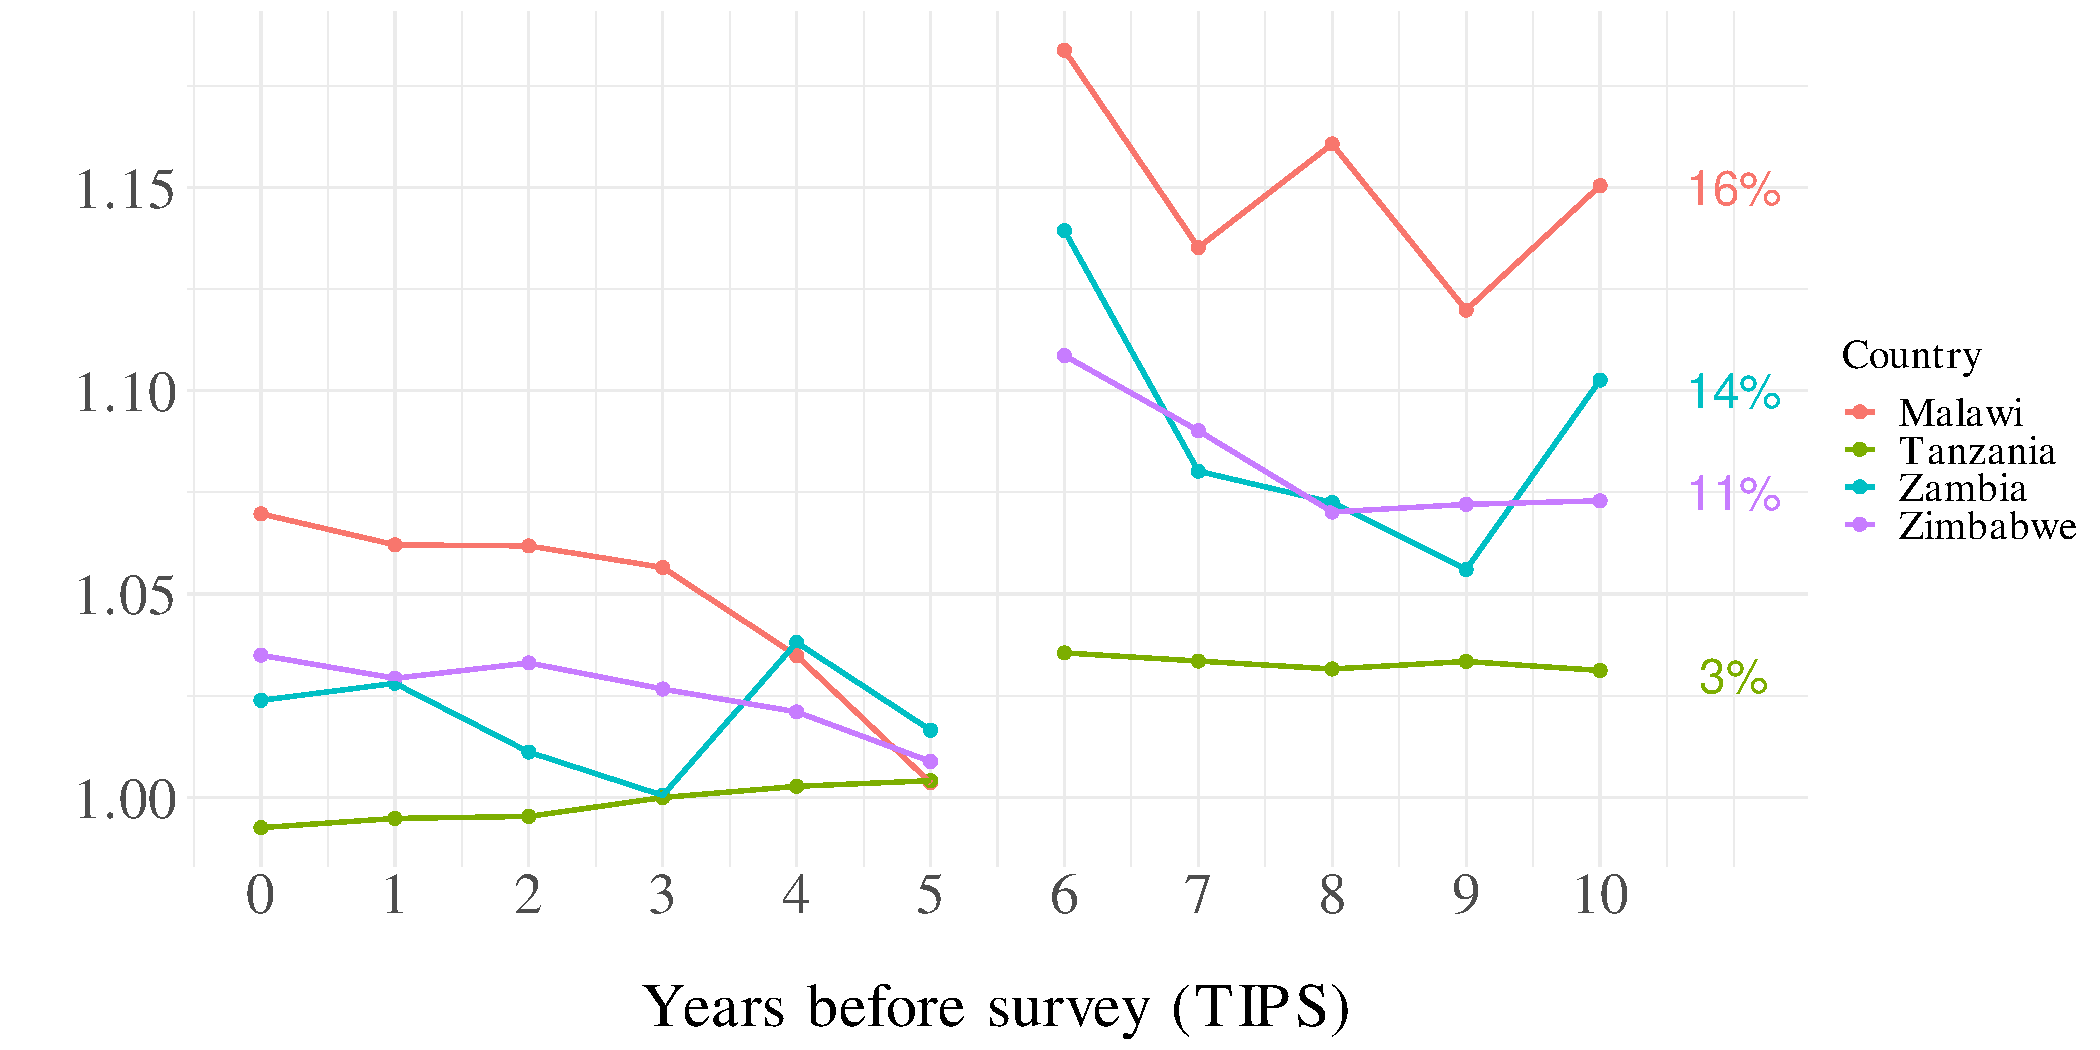
\includegraphics[height=0.5\textheight]{2020_04_UNPD_files/figure-beamer/unnamed-chunk-4-1} \end{center}

\end{frame}

\begin{frame}[t]{Model specification}
\protect\hypertarget{model-specification}{}

\[b_{ait} \sim Po( \lambda_{ait} . E_{ait} )\]
\[log(\lambda_{ait}) = \mu + \alpha_a + \gamma_t + \delta_i + \eta_{a,t} + \eta_{a,i} + \eta_{i,t}\]

\(\mu \sim N(0, 5)\)

\(\alpha_a \sim RW1(\sigma^2_\alpha)\)
\(\hfill a \in \{15-19, 20-24 ... 45-49\}\)

\(\delta_i \sim BYM2(\sigma^2_\delta)\) \(\hfill i \in \{1 ... n_i\}\)

\(\gamma_t \sim RW2(\sigma^2_\gamma)\) \(\hfill t \in \{1995:2020\}\)

\end{frame}

\begin{frame}[t]{Model specification}
\protect\hypertarget{model-specification-1}{}

\[b_{ait} \sim Po( \lambda_{ait} . E_{ait} )\]
\[log(\lambda_{ait}) = \mu + \alpha_a + \gamma_t + \delta_i + \eta_{a,t} + \eta_{a,i} + \eta_{i,t}\]

\(\eta_{a,t} \sim N(0, \sigma^2_{\eta_{a,t}})\)
\(\hfill AR1 \otimes AR1\)

\(\eta_{a,i} \sim N(0, \sigma^2_{\eta_{a,i}})\)
\(\hfill AR1 \otimes ICAR\)

\(\eta_{i,t} \sim N(0, \sigma^2_{\eta_{i,t}})\)
\(\hfill ICAR \otimes AR1\)

\end{frame}

\begin{frame}[t]{Model specification}
\protect\hypertarget{model-specification-2}{}

\[b_{ait} \sim Po( \lambda_{ait} . E_{ait} )\]
\[log(\lambda_{ait}) = \mu + \alpha_a + \gamma_t + \delta_i + \eta_{a,t} + \eta_{a,i} + \eta_{i,t}\]

Observation model
\[log(\hat{b}_{ait}) = log(\lambda_{ait} \times E_{ait}) + \beta_1 TIPS_{d} + \omega_{TIPS}\]
\(TIPS_d=\begin{cases} 0, & \text{if TIPS} < 5 \\ 1, & \text{otherwise} \end{cases}\)

\(\omega_{tips} \sim RW1(\sigma^2_\omega)\) \(\hfill tips \in \{0:14\}\)

\end{frame}

\begin{frame}{Results}
\protect\hypertarget{results}{}

tfr maps at 3 admin levels

tfr trend at admin 1

asfr from all districts in overlay plot to see distribution

\end{frame}

\begin{frame}{Future work}
\protect\hypertarget{future-work}{}

\begin{itemize}
\tightlist
\item
  Projections --\textgreater{} leontine
\item
  Survey effects - not necessarily surveyid iid, but survey type iid?
  probs not identifiable. TZA example where AIS and MIS far from DHS
\item
  Census data, other surveys, summary birth histories
\end{itemize}

\end{frame}

\end{document}
